% Options for packages loaded elsewhere
\PassOptionsToPackage{unicode}{hyperref}
\PassOptionsToPackage{hyphens}{url}
\PassOptionsToPackage{dvipsnames,svgnames*,x11names*}{xcolor}
%
\documentclass[
  12pt,
]{book}
\usepackage{lmodern}
\usepackage{setspace}
\usepackage{amssymb,amsmath}
\usepackage{ifxetex,ifluatex}
\ifnum 0\ifxetex 1\fi\ifluatex 1\fi=0 % if pdftex
  \usepackage[T1]{fontenc}
  \usepackage[utf8]{inputenc}
  \usepackage{textcomp} % provide euro and other symbols
\else % if luatex or xetex
  \usepackage{unicode-math}
  \defaultfontfeatures{Scale=MatchLowercase}
  \defaultfontfeatures[\rmfamily]{Ligatures=TeX,Scale=1}
\fi
% Use upquote if available, for straight quotes in verbatim environments
\IfFileExists{upquote.sty}{\usepackage{upquote}}{}
\IfFileExists{microtype.sty}{% use microtype if available
  \usepackage[]{microtype}
  \UseMicrotypeSet[protrusion]{basicmath} % disable protrusion for tt fonts
}{}
\makeatletter
\@ifundefined{KOMAClassName}{% if non-KOMA class
  \IfFileExists{parskip.sty}{%
    \usepackage{parskip}
  }{% else
    \setlength{\parindent}{0pt}
    \setlength{\parskip}{6pt plus 2pt minus 1pt}}
}{% if KOMA class
  \KOMAoptions{parskip=half}}
\makeatother
\usepackage{xcolor}
\IfFileExists{xurl.sty}{\usepackage{xurl}}{} % add URL line breaks if available
\IfFileExists{bookmark.sty}{\usepackage{bookmark}}{\usepackage{hyperref}}
\hypersetup{
  pdftitle={Hacia una propuesta de medición de Cohesión Social con ELSOC - Estudio Longitudinal Social de Chile / COES},
  pdfauthor={Juan Carlos Castillo, Julio Iturra \& Kevin Carrasco},
  colorlinks=true,
  linkcolor=blue,
  filecolor=Maroon,
  citecolor=Blue,
  urlcolor=Blue,
  pdfcreator={LaTeX via pandoc}}
\urlstyle{same} % disable monospaced font for URLs
\usepackage[left=4cm, right=3cm, top=2.5cm, bottom=2.5cm]{geometry}
\usepackage{longtable,booktabs}
% Correct order of tables after \paragraph or \subparagraph
\usepackage{etoolbox}
\makeatletter
\patchcmd\longtable{\par}{\if@noskipsec\mbox{}\fi\par}{}{}
\makeatother
% Allow footnotes in longtable head/foot
\IfFileExists{footnotehyper.sty}{\usepackage{footnotehyper}}{\usepackage{footnote}}
\makesavenoteenv{longtable}
\usepackage{graphicx,grffile}
\makeatletter
\def\maxwidth{\ifdim\Gin@nat@width>\linewidth\linewidth\else\Gin@nat@width\fi}
\def\maxheight{\ifdim\Gin@nat@height>\textheight\textheight\else\Gin@nat@height\fi}
\makeatother
% Scale images if necessary, so that they will not overflow the page
% margins by default, and it is still possible to overwrite the defaults
% using explicit options in \includegraphics[width, height, ...]{}
\setkeys{Gin}{width=\maxwidth,height=\maxheight,keepaspectratio}
% Set default figure placement to htbp
\makeatletter
\def\fps@figure{htbp}
\makeatother
\setlength{\emergencystretch}{3em} % prevent overfull lines
\providecommand{\tightlist}{%
  \setlength{\itemsep}{0pt}\setlength{\parskip}{0pt}}
\setcounter{secnumdepth}{5}
\usepackage[utf8]{inputenc}
\usepackage[spanish,es-tabla]{babel}
\usepackage[fixlanguage]{babelbib}
\usepackage{geometry}
\geometry{letterpaper,left=2cm,top=2cm, right=2cm}
\usepackage{times}           
\usepackage{caption}
\captionsetup[figure, table]{labelfont={bf},labelformat={default},labelsep=period}
\usepackage{graphicx}
\usepackage{float}
\usepackage{booktabs}
\usepackage{longtable}
\usepackage{array}
\usepackage{multirow}
\usepackage{wrapfig}
\usepackage{float}
\usepackage{colortbl}
\usepackage{xcolor}
\usepackage{pdflscape}
\usepackage{tabu}
\usepackage{threeparttable}
\usepackage{pdfpages} %para pdf portada

% fuente: https://stackoverflow.com/questions/45963505/coverpage-and-copyright-notice-before-title-in-r-bookdown
%\let\oldmaketitle\maketitle 
%\AtBeginDocument{\let\maketitle\relax}

% \renewcommand{\tablename}{Tabla}
% \ifxetex
%   \usepackage{polyglossia}
%   \setmainlanguage{spanish}
%   % Tabla en lugar de cuadro
%   \gappto\captionsspanish{\renewcommand{\tablename}{Tabla}
%           \renewcommand{\listtablename}{Índice de tablas}}
% \else
%   % \usepackage[spanish,es-tabla]{babel}
% \fi
\usepackage{booktabs}
\usepackage{longtable}
\usepackage{array}
\usepackage{multirow}
\usepackage{wrapfig}
\usepackage{float}
\usepackage{colortbl}
\usepackage{pdflscape}
\usepackage{tabu}
\usepackage{threeparttable}
\usepackage{threeparttablex}
\usepackage[normalem]{ulem}
\usepackage{makecell}
\usepackage{xcolor}

\title{Hacia una propuesta de medición de Cohesión Social con ELSOC - Estudio Longitudinal Social de Chile / COES}
\author{Juan Carlos Castillo, Julio Iturra \& Kevin Carrasco}
\date{2021-05-03}

\begin{document}
\maketitle

{
\hypersetup{linkcolor=}
\setcounter{tocdepth}{1}
\tableofcontents
}
\listoftables
\listoffigures
\setstretch{1.5}
\hypertarget{introducciuxf3n}{%
\chapter{Introducción}\label{introducciuxf3n}}

El objetivo de este informe es responder a un requerimiento que busca identificar los principales indicadores presentes en el Estudio Longitudinal Social de Chile (ELSOC) que permitan operacionalizar y medir el concepto de cohesión social a partir de una revisión sistemática de distintas propuestas y experiencias de estudios internacionales. Para ello, toma como principal referencia el documento de trabajo Conceptos y medición de cohesión social en proyectos internacionales de COES (Castillo et al., \protect\hyperlink{ref-castillo_Conceptos_2021}{2021}). En primer lugar, se generará una sistematización de las principales propuestas de dimensiones, subdimensiones e indicadores bajo los cuales se ha medido cohesión social a nivel internacional, señalando las principales similitudes y diferencias entre cada estudio. En segundo lugar, se analizará en qué medida las principales dimensiones y subdimensiones de cohesión social son posibles de operacionalizar con indicadores presentes en ELSOC. Para ello, se elaborarán dos insumos principales. Por un lado, una planilla que presenta la sistematización general de las dimensiones, subdimensiones e indicadores de ELSOC y la fuente de información desde dónde proviene el planteamiento de medición de la variable y, por otro lado, un documento escrito que sintetiza esta sistematización de dimensiones, subdimensiones e indicadores de manera detallada.

\hypertarget{mediciones-de-cohesiuxf3n-social-en-perspectiva-internacional}{%
\chapter{Mediciones de Cohesión social en perspectiva internacional}\label{mediciones-de-cohesiuxf3n-social-en-perspectiva-internacional}}

Este informe se basa en el documento de trabajo Conceptos y medición de cohesión social en proyectos internacionales de COES (Castillo et al., \protect\hyperlink{ref-castillo_Conceptos_2021}{2021}), en que se analizan cinco estudios internacionales que han operacionalizado distintas mediciones de cohesión social y, además, se incluye una propuesta de medición de cohesión social elaborada por un consejo asesor para el Ministerio de Desarrollo Social y Familia de Chile:

\begin{enumerate}
\def\labelenumi{\arabic{enumi})}
\item
  Mapping Social Cohesion, realizado en Canadá en 1998;
\item
  Scanlon-Monash Index of Social Cohesion, realizado en Australia desde 2007 hasta el 2019;
\item
  Social Cohesion Radar, que compara la tendencia en la cohesión social de 34 países (27 de la Unión Europea y 7 naciones industrializadas de occidente) entre 1989 y 2012;
\item
  Civic Engagement and Social Cohesion Report, realizado en Estados Unidos en 2014;
\item
  ECOsociAL, que fue realizada en siete países de América Latina (México, Guatemala, Colombia, Brasil, Perú, Argentina y Chile) en 2007.
\item
  Consejo Asesor para la Cohesión Social, realizado en Chile durante el 2020.
\end{enumerate}

Cada uno de estos estudios ha propuesto distintas definiciones de cohesión social, lo que ha implicado, a su vez, que se presenten distintas formas de operacionalización. Como resultado, se tienen distintas dimensiones, subdimensiones e indicadores que pretenden medir cohesión social. Algunas de estas dimensiones son comunes entre algunos estudios pero, en su mayoría, presentan amplias diferencias en su operacionalización, combinando indicadores que en algunos estudios se presentan como subdimensiones y en otros constituyen dimensiones. Además, las subdimensiones de distintos estudios en ocasiones se relacionan con dimensiones diferentes.

A continuación se elaborará un resumen comparativo de las distintas formas de operacionalización de mediciones de cohesión social, resaltando las similitudes y diferencias que se encuentran en cada uno de estos estudios. Las principales dimensiones que se han podido identificar de manera transversal a los diferentes estudios son: 1) Sentido de pertenencia; 2) Confianza en las instituciones; 3) Percepción de justicia; 4) Participación política; 5) Foco en el bien común; 6) Confianza; 7) Aceptación de la diversidad; 8) Redes sociales; 9) trato digno; 10) Satisfacción con la vida, felicidad y expectativas sobre el futuro; 11) Calidad de la convivencia social; y 12) Percepción de oportunidades y movilidad social.

\hypertarget{sentido-de-pertenencia}{%
\section{Sentido de pertenencia}\label{sentido-de-pertenencia}}

La dimensión denominada Sentido de Pertenencia, que aparece en Scanlon-Monash Index of Social Cohesion y en el informe del Consejo de Cohesión Social es similar a la subdimensión de Adhesión a la nación presente en ECOsociAL y una subdimensión de Identificación con la nación presente en Social Cohesion Radar. Por un lado, en el primero de estos estudios, la dimensión hace referencia a indicadores como el sentimiento de pertenencia con el país, el orgullo que siente por el país y la importancia de mantener la forma de vida y las costumbres del país. Por otro lado, en el Consejo de Cohesión Social esta dimensión sigue la propuesta realizada por el Social Cohesion Radar, el cual apunta a un aspecto más amplio de la pertenencia del país bajo una dimensión denominada Conectividad (entre individuos e instituciones o país) y que combina aspectos como la identificación con el país, la confianza en instituciones y la percepción de justicia. En el caso de ECOsociAL, presentan una dimensión denominada Calidad de la convivencia política, en que incluyen la subdimensión de Adhesión a la nación, que hace referencia a indicadores como el sentimiento de orgullo por el país y si se debe priorizar la economía nacional, la cultura nacional y los intereses del país. En este sentido, tanto en el Consejo de Cohesión Social como en el Social Cohesion Radar, la subdimensión de identificación con el país, que posee indicadores sobre sentimientos de orgullo, identificación y apego que se siente por el país, es similar a la dimensión de Sentido de Pertenencia propuesta por el Scanlon-Monash Index of Social Cohesion, mientras que en ECOsociAL solo el indicador de orgullo por el país, de la subdimensión Adhesión a la nación, es similar a esta dimensión. Sin embargo, las otras dos subdimensiones propuestas en el Social Cohesion Radar y en el Consejo de Cohesión Social y las otras cuatro subdimensiones de ECOsociAL son diferentes a la dimensión Sentido de Pertenencia de Scanlon-Monash Index of Social Cohesion.

\hypertarget{confianza-en-instituciones}{%
\section{Confianza en instituciones}\label{confianza-en-instituciones}}

La subdimensión denominada Confianza en instituciones está contenida en las dimensiones de Sentido de pertenencia del Consejo de Cohesión Social, de Conectividad en el Social Cohesion Radar y de Calidad de la convivencia política de ECOsociAL. Estas tres subdimensiones poseen indicadores similares sobre la confianza en el gobierno, la justicia o el parlamento, pero están presentes en dimensiones diferentes. Por un lado, el Consejo de Cohesión Social y el Social Cohesion Radar la agrupan en sus dimensiones de Sentido de pertenencia y de Conectividad, respectivamente, junto con dos subdimensiones de Identificación y Percepción de Justicia. Por otro lado, ECOsociAL agrupa su subdimensión de confianza en instituciones junto con las subdimensiones de Democracia y Derechos, Violencia y riesgo político, Distancia con las autoridades y Adhesión a la nación, dentro de la dimensión de Calidad de la convivencia política. La subdimensión de Democracia y Derechos, que agrupa indicadores de la calidad de integración institucional y de lealtad a la democracia, la subdimensión de Violencia y riesgo político, que agrupa indicadores de riesgo político observado y legitimación de la violencia y la subdimensión de Distancia con las autoridades, que agrupa indicadores de identificación y hostilidad hacia el gobierno, sólo están presentes en ECOsociAL.

\hypertarget{percepciuxf3n-de-justicia}{%
\section{Percepción de justicia}\label{percepciuxf3n-de-justicia}}

La subdimensión de Percepción de justicia de la dimensión Conectividad de Social Cohesion Radar agrupa indicadores sobre corrupción, sobre si se recibe un sueldo justo y la opinión sobre si el gobierno debería reducir las diferencias en los niveles de ingresos. El Consejo de Cohesión Social incluye una subdimensión del mismo nombre en su dimensión Sentido de pertenencia, en la que utiliza indicadores de corrupción e incluye indicadores sobre la percepción de injusticia en el acceso a salud y educación, percepción de las diferencias de ingresos, si las personas son recompensadas por sus esfuerzos, la importancia del trabajo duro para surgir en la vida y si el gobierno toma en consideración el punto de vista de las personas para diseñar políticas públicas. Por un lado, los indicadores de percepción de injusticia en el acceso a salud y a educación es similar a las subdimensiones de Mapping Social Cohesion de Acceso a educación y capital humano y Acceso a la salud, que incluyen indicadores estructurales como la tasa de alfabetización, porcentaje de población que ha completado educación secundaria, la esperanza de vida al nacer o mortalidad infantil. Sin embargo, la dimensión de disparidades sociales de Mapping Social Cohesion también incluye otras subdimensiones sobre acceso a recursos financieros, acceso a tecnología y de inclusión en la actividad económica. Por otro lado, los indicadores de percepción de las diferencias de ingresos y de la importancia del trabajo duro para surgir en la vida de la subdimensión de Sentido de pertenencia del Consejo de Cohesión Social son similares a la dimensión de Equidad y justicia social de Scanlon-Monash Index of Social cohesion, en que se incluyen estos dos indicadores junto con la percepción de que las personas con bajos ingresos reciben suficiente apoyo y si el gobierno hace las cosas correctas por las personas.

\hypertarget{participaciuxf3n-poluxedtica}{%
\section{Participación política}\label{participaciuxf3n-poluxedtica}}

Scanlon-Monash Index of Social Cohesion presenta una dimensión de Participación política, en que incluye indicadores sobre votar en elecciones, firmar una petición, asistir a una protesta o el contacto con miembros del parlamento. En Mapping Social Cohesion se presenta una subdimensión similar denominada Participación y solidaridad, en que se combinan indicadores sobre participación electoral, participación en asociaciones voluntarias y caridad. Asimismo, Social Cohesion Radar y el Consejo de Cohesión Social incluyen una subdimensión denominada Participación cívica, en que incluyen indicadores sobre participación en elecciones, interés en política, asistir a manifestaciones y trabajo en organizaciones sociales. En este sentido, si bien estas tres últimas subdimensiones son similares entre sí, están incluidas en dimensiones diferentes. La subdimensión de Participación y solidaridad de Mapping Social Cohesion se presenta en conjunto con una subdimensión de Confianza, en una dimensión denominada Mediciones de pertenencia y participación, mientras que la subdimensión de Participación cívica de Social Cohesion Radar y del Consejo de Cohesión Social se presenta junto a dos subdimensiones, una de Solidaridad y amabilidad, en la cual se incluye un indicador de trabajo en actividades de voluntariado y una de Respeto por las normas sociales, dentro de una dimensión denominada Foco en el bien común.

\hypertarget{foco-en-el-bien-comuxfan}{%
\section{Foco en el bien común}\label{foco-en-el-bien-comuxfan}}

En Social Cohesion Radar y en el Consejo de Cohesión social, dentro de su dimensión Foco en el bien común incluyen, por un lado, una subdimensión denominada Respeto por las normas sociales. En Social Cohesion Radar esta subdimensión incluye indicadores sobre cuán malo es cometer una infracción de tráfico, el tamaño de la economía informal y la sensación de seguridad caminando solo por la noche, mientras que en el Consejo de Cohesión Social esta subdimensión incluye un indicador de temor a caminar solo en la noche en su barrio y temor a ser acosado sexualmente en su lugar de trabajo o estudio. Por otro lado, Social Cohesion Radar incluye una subdimensión denominada Solidaridad y amabilidad, que incluye indicadores de ayuda a extraños, trabajo voluntario y dinero donado, mientras que en el Consejo de Cohesión Social esta subdimensión se denomina Solidaridad y ayuda e incluye indicadores de percepción sobre si el gobierno debería subir impuestos a los más ricos para ayudar a los pobres, disposición a pagar impuestos para mejorar atención en salud y indicadores de donar dinero y participar en actividades de voluntariado.

\hypertarget{confianza-social}{%
\section{Confianza social}\label{confianza-social}}

Como se mencionó anteriormente, en Mapping Social Cohesion se presenta una dimensión de mediciones de pertenencia y participación, que posee una subdimensión de Confianza que incluye indicadores sobre confianza en las personas a partir de encuesta de opinión pública. Esta subdimensión es similar a la subdimensión de Confianza en las personas que presentan Social Cohesion Radar y el Consejo de Cohesión Social, que incluye indicadores sobre la confianza social generalizada, de percepción sobre si las personas intentan ser justas y sobre altruismo social y que se incluye en una dimensión denominada Calidad del vínculo social. De la misma forma, esta subdimensión es similar a la subdimensión de Confianza social presentada por ECOsociAL, que incluye indicadores sobre si se puede confiar en las personas y si la mayoría de las personas actúa correctamente, la que se incluye en una dimensión más amplia denominada Calidad de la convivencia social. Si bien estas subdimensiones son similares, nuevamente se presentan insertas en dimensiones distintas.

\hypertarget{aceptaciuxf3n-de-la-diversidad}{%
\section{Aceptación de la diversidad}\label{aceptaciuxf3n-de-la-diversidad}}

En Scanlon Monash Index of Social Cohesion se propone una dimensión de Aceptación y rechazo, en que se incluyen indicadores de experiencias de discriminación en base a color de piel, etnia o religión, de pesimismo sobre el futuro, si cree que el gobierno debe dar asistencia para que las minorías étnicas mantengan sus costumbres y si cree que aceptar inmigrantes hace al país más fuerte. Por su parte, en Social cohesion radar se propone una subdimensión de Aceptación de la diversidad, que incluye indicadores de la percepción sobre si la cultura del país es socavada por los inmigrantes, si la ciudad es un buen lugar para minorías raciales o étnicas o para gays y lesbianas, si gays y lesbianas son libres de vivir su vida como deseen y la tensión religiosa existente. En el Consejo de Cohesión social se propone una subdimensión del mismo nombre, que incluye indicadores sobre percepción del aporte positivo y negativo de la migración, del derecho a casarse y de adopción de las parejas homosexuales y si se debe reconocer constitucionalmente a Chile como un país multicultural. En ECOsociAL se propone una subdimensión similar de Tolerancia y Discriminación, donde se incluyen indicadores de sentimientos de exclusión, como si lo que la persona piense no le importa a los demás, si lo dejan al margen de cosas que ocurren a su alrededor o si la gente haría poco para ayudarlo, un indicador de la frecuencia con que ha sido discriminado por color de piel, raza o etnia, religión, condición de pobreza o preferencia política, indicadores de tolerancia como situaciones en que sus hijos tienen un amigo homosexual, se casan con alguien de una clase social más baja o con alguien que no tiene religión, o sobre tener vecinos de una clase social más baja, inmigrantes o de otra raza, e indicadores sobre homogamia en relación con etnia, religión y educación. En el caso de Social Cohesion Radar y el Consejo de Cohesión social esta subdimensión se presenta dentro de la dimensión de Calidad del vínculo social, mientras que en ECOsociAL está dentro de la dimensión Calidad de la convivencia social. Finalmente, Mapping Social cohesion incluye una dimensión de homogeneidad cultural y étnica, en que incluyen indicadores del porcentaje de extranjeros en la población y de fraccionalización étnica.

\hypertarget{redes-sociales}{%
\section{Redes sociales}\label{redes-sociales}}

Dentro de la dimensión Calidad del vínculo social de Social Cohesion Radar se incluye una subdimensión de Redes sociales, que incluye indicadores sobre con qué frecuencia se reúne socialmente con amigos, familiares o colegas, cuánto tiempo durante la semana se sintió solo, si cuenta con ayuda y si cuenta con apoyo si necesita consejos. Esta subdimensión se presenta de manera similar en el Consejo de cohesión social bajo el nombre de Relaciones sociales, que posee indicadores sobre la cantidad de amistades cercanas, el contacto presencial con amistades y con vecinos y las redes de apoyo para obtener un préstamo y para conversar sobre temas importantes. En Civic Engagement and Social cohesion report se incluye una dimensión de nivel individual que posee indicadores sobre la presencia de redes de apoyo, de participación en grupos de chat online y de la frecuencia de interacción con familia o amigos, de las veces que ha recibido ayuda de familia o amigos y la frecuencia con que ha sentido soledad. Asimismo, en ECOsociAL se presenta una subdimensión denominada Relaciones de amistad, vecindad y asociatividad, que incluye indicadores de asociatividad a partir de participación en organizaciones sociales y relaciones de amistad y vecindad a partir del número de amigos y vecinos que se conocen por su nombre y la frecuencia de contactos con ellos.

\hypertarget{trato-digno}{%
\section{Trato digno}\label{trato-digno}}

El Consejo de Cohesión Social, dentro de la dimensión de Calidad del vínculo social, incluye una subdimensión de Trato digno, que posee indicadores sobre las experiencias de haber recibido malos tratos en sus diversas expresiones y, específicamente, en los servicios de salud y en las oficinas del servicio público y la percepción de conflictividad percibida entre clases bajas y altas.

\hypertarget{satisfacciuxf3n-con-la-vida-felicidad-y-expectativas-sobre-el-futuro.}{%
\section{Satisfacción con la vida, felicidad y expectativas sobre el futuro.}\label{satisfacciuxf3n-con-la-vida-felicidad-y-expectativas-sobre-el-futuro.}}

En Scanlon-Monash Index of social cohesion se presenta una dimensión denominada valoración, que posee subdimensiones de satisfacción con la situación financiera y de felicidad en los últimos años, que incluyen indicadores de satisfacción con la situación económica y de satisfacción con la vida, felicidad y de expectativas sobre el futuro.

\hypertarget{calidad-de-la-convivencia-social.}{%
\section{Calidad de la convivencia social.}\label{calidad-de-la-convivencia-social.}}

Dentro de la dimensión Calidad de la convivencia social de ECOsociAL se presenta una subdimensión de solidaridad familiar, que incluye indicadores de la calidad de relación con la familia; una subdimensión de solidaridad intergeneracional, que posee indicadores de la relación padres-hijos; una subdimensión de Calidad de la vida de barrio, que posee indicadores de vandalismo, robos y asaltos; una subdimensión de Victimización, que posee indicadores de reportes de victimización por robo y de intimidación con arma de fuego; y una subdimensión de Temor, que posee indicadores de declaraciones de temor para cuando se está solo en la casa o caminando por el barrio durante la noche.

\hypertarget{percepciuxf3n-de-oportunidades-y-movilidad-social.}{%
\section{Percepción de oportunidades y movilidad social.}\label{percepciuxf3n-de-oportunidades-y-movilidad-social.}}

ECOsociAL propone una dimensión de Percepción de oportunidades y movilidad social, que posee las siguientes subdimensiones: Percepción de oportunidades; identificación socioeconómica; oportunidades de vulnerabilidad; Movilidad social; Legitimación de diferencias socioeconómicas; y Desigualdad.

\hypertarget{dimensiones-comunes-entre-los-estudios-internacionales-e-indicadores-presentes-en-elsoc}{%
\chapter{Dimensiones comunes entre los estudios internacionales e indicadores presentes en ELSOC}\label{dimensiones-comunes-entre-los-estudios-internacionales-e-indicadores-presentes-en-elsoc}}

\hypertarget{sentido-de-pertenencia-1}{%
\section{Sentido de pertenencia}\label{sentido-de-pertenencia-1}}

En ELSOC los indicadores que miden esta dimensión son los pertenecientes al concepto de Identidad nacional, del módulo de Sociabilidad Política, y que preguntan por el grado de acuerdo o en desacuerdo con las siguientes dos afirmaciones: 1) Me identifico con Chile; y 2) Me siento orgulloso de ser chileno/a. En relación con la primera afirmación, esta también ha sido utilizada por el Consejo de Cohesión social, mientras que la segunda afirmación ha sido utilizada por Scanlon-Monash Index of Social Cohesion.

\hypertarget{confianza-en-instituciones.}{%
\section{Confianza en instituciones.}\label{confianza-en-instituciones.}}

En ELSOC los indicadores que miden esta dimensión se encuentran en el módulo Ciudadanía y Democracia, bajo el concepto de Confianza en instituciones que pregunta sobre el grado de confianza hacia 1) El congreso nacional; 2) Los partidos políticos; 3) Fiscalía Nacional; 4) El poder judicial; 5) Carabineros; 6) Fuerzas armadas; 7) El gobierno; 8) Su municipalidad; 9) Los sindicatos; 10) Las empresas privadas; 11) El presidente de la república; 12) Bomberos; y 13) Medios de comunicación tradicionales. De estos indicadores, los primeros seis han sido utilizados por Social Cohesion Radar y por el Consejo de cohesión social, mientras que los indicadores 7 y 8 han sido utilizados por ECOsociAL. Los últimos cinco indicadores no han sido utilizados en ningún estudio.

Además, dentro de esta dimensión se incluye una subdimensión de Lealtad hacia la democracia que, en ELSOC, el indicador que sirve para medir lealtad hacia la democracia se encuentra en el módulo de Ciudadanía y democracia, bajo el concepto de Actitud hacia la democracia, que pregunta sobre cuán satisfecho o insatisfecho se encuentra con el funcionamiento de la democracia en Chile. Este indicador específico no ha sido utilizado en ningún estudio previo. Sin embargo, ECOsociAL propone una subdimensión denominada Lealtad hacia la Democracia que pregunta si la democracia es mejor a cualquier otra forma de gobierno y si los derechos de las personas se deben respetar en toda circunstancia.

\hypertarget{percepciuxf3n-de-justicia-1}{%
\section{Percepción de justicia}\label{percepciuxf3n-de-justicia-1}}

En ELSOC los indicadores que miden corrupción se encuentran en el módulo Ciudadanía y Democracia. El primero bajo el concepto de Anomia, que pregunta sobre el grado de acuerdo con que para que a uno le vaya bien en nuestro país, a veces es necesario hacer trampa y el segundo bajo el concepto de Percepción de corrupción, que pregunta sobre en qué medida la corrupción en la política está extendida en Chile. El primero de estos indicadores es utilizado en Social Cohesion Radar y el segundo es utilizado en el Consejo de cohesión social.

Los indicadores que miden si se recompensa el esfuerzo y la importancia del trabajo duro para surgir en la vida se encuentran en el módulo de Sociabilidad política, bajo el concepto de Justicia distributiva y meritocracia, que preguntan sobre el grado de acuerdo o en desacuerdo con que en Chile las personas son recompensadas por sus esfuerzos y por su inteligencia y habilidades. Estos dos indicadores han sido utilizados por el Consejo de cohesión social, mientras que indicadores similares han sido utilizados por Social Cohesion Radar, ECOsociAL y Scanlon-Monash Index of Social Cohesion. Otros indicadores presentes en ELSOC que podrían servir para medir esta subdimensión se encuentran en el módulo de Desigualdad y legitimidad, bajo el concepto de Surgir en la vida, y que preguntan sobre cuán importante es para surgir en la vida: 1) provenir de una familia rica o con muchos recursos; 2) tener un buen nivel de educación; 3) tener ambición; y 4) el trabajo duro.

Un indicador que mide la percepción de las diferencias de ingresos se encuentra en el módulo de Sociabilidad política, bajo el concepto de Desigualdad percibida, que pregunta sobre el grado de acuerdo o en desacuerdo con que en Chile las diferencias de ingresos son demasiado grandes. Otro indicador, que mide esta subdimensión se encuentra en el módulo Desigualdad y legitimidad, bajo el concepto de Conflicto de clase, que pregunta sobre cuán justa o injusta es la diferencia en la situación de vida entre las personas de clase alta y las de clase social baja en Chile. De estos indicadores solo el primero ha sido utilizado por el Consejo de Cohesión social, mientras que el segundo indicador presenta una versión similar en Scanlon-Monash Index of Social Cohesion, que pregunta por el grado de acuerdo con que existe una gran diferencia en ingresos. Asimismo, ELSOC presenta tres indicadores que podrían ser utilizados para medir esta subdimensión en el módulo de Sociabilidad política, bajo el concepto de Dominancia Social, que pregunta sobre el grado de acuerdo con las siguientes afirmaciones: 1) Una sociedad ideal requiere que algunos grupos estén en una posición superior y otros en una posición inferior; 2) Debiéramos trabajar para dar a todos los grupos la misma oportunidad de tener éxito; y 3) Deberíamos hacer todo lo posible por igualar las condiciones de diferentes grupos.

\hypertarget{participaciuxf3n-poluxedtica-1}{%
\section{Participación política}\label{participaciuxf3n-poluxedtica-1}}

En ELSOC los principales indicadores que miden esta dimensión se encuentran en el módulo de Ciudadanía y Democracia, bajo el concepto de Participación ciudadana, que pregunta si votó en las últimas elecciones presidenciales, su grado de interés en la política y por la frecuencia con que 1) ha firmado una carta o petición; 2) Asistido a una marcha o manifestación pacífica; 3) participado en una huelga; 4) Usado las redes sociales para expresar su opinión en temas públicos; y 5) Participado en cacerolazos. Por un lado, el primer indicador sobre participación electoral está presente en Mapping Social Cohesion, Scanlon-Monash Index of Social Cohesion, Social Cohesion Radar y en el Consejo de Cohesión Social y el grado de interés en la política ha sido utilizado en Social Cohesion Radar y en el Consejo de Cohesión Social. Por otro lado, en cuanto a la frecuencia de participación ciudadana, el indicador sobre firmar una carta o petición ha sido utilizado por Scanlon-Monash Index of Social Cohesion y Social Cohesion Radar y el indicador sobre asistir a una marcha o manifestación ha sido utilizado por Scanlon-Monash Index of Social Cohesion y por el Consejo de cohesión social, mientras que los otros tres indicadores de frecuencia de participación ciudadana no se han utilizado en ninguno de los estudios revisados. En esta línea, el concepto de Participación ciudadana de ELSOC también incluye indicadores sobre la participación en las siguientes organizaciones voluntarias: 1) Juntas de vecinos u otra organización vecinal; 2) Organización religiosa; 3) Partido o movimiento político; 4) Sindicato; 5) Asociación profesional o gremial; 6) Organización deportiva; 7) Organización ecológica o medioambiental; y 7) asociaciones o centros de estudiantes. Este conjunto de organizaciones se agrupan en un solo indicador de Social Cohesion Radar y del Consejo de Cohesión Social que pregunta sobre la participación y trabajo en asociaciones u organizaciones sociales.

\hypertarget{foco-en-el-bien-comuxfan-1}{%
\section{Foco en el bien común}\label{foco-en-el-bien-comuxfan-1}}

En ELSOC los indicadores que miden solidaridad se encuentran en el módulo Sociabilidad política y preguntan sobre la frecuencia con que 1) Ha hecho voluntariado y 2) ha donado dinero a una obra social o de caridad. Este primer indicador ha sido utilizado por Mapping Social Cohesion, Social Cohesion Radar y el Consejo de cohesión social, mientras que el segundo ha sido solo utilizado por Social Cohesion Radar y por el Consejo de Cohesión social. Asimismo, ELSOC incluye otros indicadores dentro del módulo Sociabilidad política que podrían ser útiles para medir esta subdimensión pero que no han sido utilizados por otras organizaciones. Estos abordan la frecuencia con que 1) Ha prestado una suma de dinero de \$10.000.- o más; 2) Ha conversado con una persona en problemas o deprimida; y 3) Ha ayudado a alguien a conseguir trabajo.

\hypertarget{confianza-social-1}{%
\section{Confianza social}\label{confianza-social-1}}

En ELSOC un indicador que mide esta dimensión es el perteneciente al concepto de Confianza en vecinos, del módulo Territorio, que aborda, en términos generales, cuánto confía la persona en sus vecinos, que es similar a los indicadores pertenecientes a Mapping Social Cohesion, Social Cohesion Radar y el Consejo de Cohesión Social. Otros indicadores son los pertenecientes al concepto de Confianza interpersonal, del módulo Ciudadanía y Democracia, que preguntan sobre 1) si la mayoría de las veces las personas tratan de ayudar a los demás o se preocupan mayormente solo de sí mismas; 2) si se puede confiar en la mayoría de las personas o hay que tener cuidado al tratar con ellas; y 3) si cree que la mayoría de la gente intentaría aprovecharse de usted si tuviera la oportunidad o cree que trataría de ser justa. El primer indicador ha sido utilizado en el Consejo de Cohesión social, mientras que los dos últimos han sido utilizados en
ECOsociAL.

\hypertarget{aceptaciuxf3n-de-la-diversidad-1}{%
\section{Aceptación de la diversidad}\label{aceptaciuxf3n-de-la-diversidad-1}}

Un indicador de ELSOC, que también ha sido utilizado por el Consejo de Cohesión Social, es el grado de acuerdo o en desacuerdo con que las parejas homosexuales deberían poder adoptar hijos. Existen otros indicadores de ELSOC que apuntan en una dirección similar a lo planteado en esta dimensión, pero que no han sido utilizados directamente por ninguna otra organización. Estos son el grado de acuerdo o en desacuerdo con que: 1) Chile debiera fomentar la migración de {[}peruanos/venezolanos{]} altamente calificados; 2) los migrantes {[}peruanos/venezolanos{]} deben tener el mismo acceso a los servicios de salud pública que los chilenos; 3) Es importante para mí que los peruanos que viven en Chile mantengan sus costumbres y tradiciones.; 4) Es importante para mí que los peruanos que viven en Chile adquieran la forma de vida de los chilenos; 5) Con la llegada de tantos peruanos, Chile está perdiendo su identidad; y 6) Con la llegada de tantos peruanos a Chile está aumentando el desempleo.

\hypertarget{redes-sociales-1}{%
\section{Redes sociales}\label{redes-sociales-1}}

En ELSOC el principal indicador que mide esta dimensión es el tamaño de la red cercana, presente en el módulo de Redes y Actitudes. Este indicador también está presente en ECOsociAL y en el Consejo de Cohesión Social.

\hypertarget{trato-digno-1}{%
\section{Trato digno}\label{trato-digno-1}}

Los indicadores que miden la dimensión de Trato digno se encuentran en el módulo de Sociabilidad política. Un indicador, que también ha sido utilizado en el Consejo de Cohesión Social, corresponde a la frecuencia con que las personas son tratadas con respeto en los servicios de salud. Además, en este módulo se incluyen otros tres indicadores que no han sido utilizados en otro estudio y que preguntan sobre la frecuencia con que las personas son tratadas con respeto en el trabajo, por carabineros y por personas de clase alta.
El principal indicador que mide Tensión entre clases se encuentra en el módulo de Conflicto social, que pregunta sobre el conflicto percibido entre personas de clase alta y personas de clase baja. Un indicador similar ha sido utilizado por el Consejo de cohesión social, mientras que en Social Cohesion Radar se pregunta sobre la tensión entre ricos y pobres y en ECOsociAL se pregunta sobre la identificación y hostilidad con la clase baja, media y alta.

\hypertarget{satisfacciuxf3n-con-la-vida-felicidad-y-expectativas-sobre-el-futuro.-1}{%
\section{Satisfacción con la vida, felicidad y expectativas sobre el futuro.}\label{satisfacciuxf3n-con-la-vida-felicidad-y-expectativas-sobre-el-futuro.-1}}

En ELSOC el indicador que mide esta dimensión se encuentra en el módulo Salud y Bienestar, que pregunta sobre el grado de satisfacción o insatisfacción con la vida en este momento. Este indicador también ha sido utilizado en Scanlon-Monash Index of Social Cohesion.

\hypertarget{calidad-de-la-convivencia-social.-1}{%
\section{Calidad de la convivencia social.}\label{calidad-de-la-convivencia-social.-1}}

En ELSOC los indicadores que miden esta dimensión se encuentran dentro del módulo Territorio y preguntan sobre la frecuencia con que se han producido 1) robos o asaltos a personas, casas y/o vehículos; 2) riñas o peleas callejeras; 3) amenazas, insultos u ofensas de parte de vecinos de su barrio y 4) qué tan seguro o inseguro se siente en el barrio o vecindario en que la persona vive. Los tres primeros indicadores han sido utilizados por ECOsociAL, mientras que el cuarto ha sido utilizado por el Consejo de Cohesión Social. Asimismo, ELSOC incluye otros indicadores que podrían ser útiles para medir esta subdimensión pero que no han sido utilizados por otras organizaciones. Estos son indicadores de problemas de convivencia con los vecinos, de integración y pertenencia al vecindario y de satisfacción con el vecindario; todos ellos pertenecientes al módulo Territorio.

\hypertarget{percepciuxf3n-de-oportunidades-y-movilidad-social.-1}{%
\section{Percepción de oportunidades y movilidad social.}\label{percepciuxf3n-de-oportunidades-y-movilidad-social.-1}}

En ELSOC un indicador que mide percepción de oportunidades se encuentra en el módulo Sociabilidad política, que pregunta sobre el grado de acuerdo o en desacuerdo con que en Chile las personas tienen igualdad de oportunidades para salir adelante. Si bien este indicador específico no ha sido utilizado en otro estudio, en ECOsociAL se pregunta sobre la percepción de oportunidades educativas y de bienestar.

Los indicadores que miden movilidad social se encuentran en el módulo Desigualdad y legitimidad bajo el concepto de Estatus subjetivo que, bajo la premisa de que en nuestra sociedad hay grupos que tienden a ubicarse en los niveles más altos y grupos que tienden a ubicarse en los niveles más bajos de la sociedad, pregunta sobre en qué posición se ubicaría en la sociedad chilena, dónde ubicaría la familia en la que creció y dónde cree que se ubicarán sus hijos. Tres indicadores similares han sido utilizados por ECOsociAL, que incluye la comparación del nivel educacional de los padres con el encuestado, la comparación entre su posición actual y hace diez años y la comparación entre el encuestado y sus hijos.

\hypertarget{propuesta-de-mediciuxf3n-de-cohesiuxf3n-social-con-indicadores-de-elsoc}{%
\chapter{Propuesta de medición de Cohesión Social con indicadores de ELSOC}\label{propuesta-de-mediciuxf3n-de-cohesiuxf3n-social-con-indicadores-de-elsoc}}

La siguiente propuesta de medición de cohesión social agrupa los principales indicadores de ELSOC en dos dimensiones. Por un lado, se abarca un aspecto más general de la cohesión social al intentar aunar distintos indicadores que miden una vinculación vertical de los individuos con las instituciones y con el funcionamiento del país. Por otro lado, se agrupan indicadores más específicos que miden una vinculación horizontal de los individuos con el territorio y con otros individuos. Todos los indicadores de esta propuesta de medición están presentes en las cuatro olas de ELSOC (2016-2019)

\begin{table}[!h]

\caption{\label{tab:unnamed-chunk-5}Medición de cohesión social con ELSOC.}
\centering
\fontsize{10}{12}\selectfont
\begin{tabu} to \linewidth {>{\raggedright\arraybackslash}p{2 cm}>{\raggedright\arraybackslash}p{2 cm}>{\raggedright\arraybackslash}p{4 cm}>{\raggedright\arraybackslash}p{2 cm}>{\raggedright\arraybackslash}p{3 cm}>{\raggedright\arraybackslash}p{2 cm}}
\toprule
Dimensión & Subdimensión & Encabezado & Indicador & Categoría de respuesta & Código ELSOC\\
\midrule
 &  & “Utilizando una escala donde 1 representa "Nada" y 5 "Mucha", ¿podría decirme cuánto confía usted en cada una de las siguientes instituciones?” & El gobierno & No Responde (no leer)|No Sabe (no leer)|Nada|Poca|Algo|Bastante|Mucha & c05\_01\\
\cmidrule{3-6}
 &  & “Utilizando una escala donde 1 representa "Nada" y 5 "Mucha", ¿podría decirme cuánto confía usted en cada una de las siguientes instituciones?” & Los partidos políticos & No Responde (no leer)|No Sabe (no leer)|Nada|Poca|Algo|Bastante|Mucha & c05\_02\\
\cmidrule{3-6}
 &  & “Utilizando una escala donde 1 representa "Nada" y 5 "Mucha", ¿podría decirme cuánto confía usted en cada una de las siguientes instituciones?” & Carabineros & No Responde (no leer)|No Sabe (no leer)|Nada|Poca|Algo|Bastante|Mucha & c05\_03\\
\cmidrule{3-6}
 &  & “Utilizando una escala donde 1 representa "Nada" y 5 "Mucha", ¿podría decirme cuánto confía usted en cada una de las siguientes instituciones?” & Los sindicatos & No Responde (no leer)|No Sabe (no leer)|Nada|Poca|Algo|Bastante|Mucha & c05\_04\\
\cmidrule{3-6}
 &  & “Utilizando una escala donde 1 representa "Nada" y 5 "Mucha", ¿podría decirme cuánto confía usted en cada una de las siguientes instituciones?” & El poder judicial & No Responde (no leer)|No Sabe (no leer)|Nada|Poca|Algo|Bastante|Mucha & c05\_05\\
\cmidrule{3-6}
 &  & “Utilizando una escala donde 1 representa "Nada" y 5 "Mucha", ¿podría decirme cuánto confía usted en cada una de las siguientes instituciones?” & Las empresas privadas & No Responde (no leer)|No Sabe (no leer)|Nada|Poca|Algo|Bastante|Mucha & c05\_06\\
\cmidrule{3-6}
 &  & “Utilizando una escala donde 1 representa "Nada" y 5 "Mucha", ¿podría decirme cuánto confía usted en cada una de las siguientes instituciones?” & El congreso nacional & No Responde (no leer)|No Sabe (no leer)|Nada|Poca|Algo|Bastante|Mucha & c05\_07\\
\cmidrule{3-6}
 & \multirow{-8}{2 cm}{\raggedright\arraybackslash Confianza en instituciones} & “Utilizando una escala donde 1 representa "Nada" y 5 "Mucha", ¿podría decirme cuánto confía usted en cada una de las siguientes instituciones?” & El presidente(a) de la república & No Responde (no leer)|No Sabe (no leer)|Nada|Poca|Algo|Bastante|Mucha & c05\_08\\
\cmidrule{2-6}
\multirow{-9}{2 cm}{\raggedright\arraybackslash Confianza en instituciones y satisfacción con la democracia} & Actitud (satisfacción) hacia la democracia & ¿Cuán satisfecho o insatisfecho está usted con el funcionamiento de la democracia en Chile? &  & No Responde (no leer)|No Sabe (no leer)|Nada satisfecho|Poco satisfecho|Algo satisfecho|Bastante satisfecho|Muy satisfecho & c01\\
\cmidrule{1-6}
 &  & “Durante los últimos 12 meses,  con cuánta frecuencia usted ha ...” & Firmado una carta o petición apoyando una causa & No Responde (no leer)|No Sabe (no leer)|Nunca|Casi nunca|A veces|Frecuentemente|Muy frecuentemente & c08\_01\\
\cmidrule{3-6}
 &  & “Durante los últimos 12 meses,  con cuánta frecuencia usted ha ...” & Asistido a una marcha o manifestación política & No Responde (no leer)|No Sabe (no leer)|Nunca|Casi nunca|A veces|Frecuentemente|Muy frecuentemente & c08\_02\\
\cmidrule{3-6}
 &  & “Durante los últimos 12 meses,  con cuánta frecuencia usted ha ...” & Participado en una huelga & No Responde (no leer)|No Sabe (no leer)|Nunca|Casi nunca|A veces|Frecuentemente|Muy frecuentemente & c08\_03\\
\cmidrule{3-6}
 & \multirow{-4}{2 cm}{\raggedright\arraybackslash Participación ciudadana} & “Durante los últimos 12 meses,  con cuánta frecuencia usted ha ...” & Usado las redes sociales para expresar su opinión en temas público & No Responde (no leer)|No Sabe (no leer)|Nunca|Casi nunca|A veces|Frecuentemente|Muy frecuentemente & c08\_04\\
\cmidrule{2-6}
 &  & ¿Qué tan interesado está usted en la política? &  & No Responde (no leer)|No Sabe (no leer)|Nada interesado|Poco interesado|Algo interesado|Bastante interesado|Muy interesado & c13\\
\cmidrule{3-6}
 &  & ¿Con qué frecuencia realiza usted las siguientes actividades? & Habla de política con familiares o amigos & No Responde (no leer)|No Sabe (no leer)|Nunca|Casi nunca|A veces|Frecuentemente|Muy frecuentemente & c14\_01\\
\cmidrule{3-6}
\multirow{-7}{2 cm}{\raggedright\arraybackslash Participación política} & \multirow{-3}{2 cm}{\raggedright\arraybackslash Interés político} & ¿Con qué frecuencia realiza usted las siguientes actividades? & Se informa activamente sobre política en medios tales como televisión, radios, diarios o internet & No Responde (no leer)|No Sabe (no leer)|Nunca|Casi nunca|A veces|Frecuentemente|Muy frecuentemente & c14\_02\\
\cmidrule{1-6}
 &  & ¿En qué medida se encuentra usted de acuerdo o en desacuerdo con cada una de las siguientes afirmaciones? & En Chile las personas son recompensadas por sus esfuerzos & No Responde (no leer)|No Sabe (no leer)|Totalmente en desacuerdo|En desacuerdo|Ni en desacuerdo ni de acuerdo|De acuerdo|Totalmente de acuerdo & c18\_09\\
\cmidrule{3-6}
 & \multirow{-2}{2 cm}{\raggedright\arraybackslash Justicia distributiva y meritocracia} & ¿En qué medida se encuentra usted de acuerdo o en desacuerdo con cada una de las siguientes afirmaciones? & En Chile las personas son recompensadas por su inteligencia y habilidades & No Responde (no leer)|No Sabe (no leer)|Totalmente en desacuerdo|En desacuerdo|Ni en desacuerdo ni de acuerdo|De acuerdo|Totalmente de acuerdo & c18\_10\\
\cmidrule{2-6}
 &  & Actualmente en Chile, ¿Cuán importante es para surgir en la vida…? & Provenir de una familia rica o con muchos recursos & No Responde (no leer)|No Sabe (no leer)|Nada Importante|Poco importante|Algo importante|Bastante importante|Muy importante & d05\_01\\
\cmidrule{3-6}
 &  & Actualmente en Chile, ¿Cuán importante es para surgir en la vida…? & Tener un buen nivel de educación & No Responde (no leer)|No Sabe (no leer)|Nada Importante|Poco importante|Algo importante|Bastante importante|Muy importante & d05\_02\\
\cmidrule{3-6}
 &  & Actualmente en Chile, ¿Cuán importante es para surgir en la vida…? & Tener ambición & No Responde (no leer)|No Sabe (no leer)|Nada Importante|Poco importante|Algo importante|Bastante importante|Muy importante & d05\_03\\
\cmidrule{3-6}
\multirow{-6}{2 cm}{\raggedright\arraybackslash Percepción de justicia (distributiva)} & \multirow{-4}{2 cm}{\raggedright\arraybackslash Surgir en la vida} & Actualmente en Chile, ¿Cuán importante es para surgir en la vida…? & El trabajo duro & No Responde (no leer)|No Sabe (no leer)|Nada Importante|Poco importante|Algo importante|Bastante importante|Muy importante & d05\_04\\
\cmidrule{1-6}
 & Confianza en vecinos & En términos generales, ¿cuánto confía usted en sus vecinos? &  & No Responde (no leer)|No Sabe (no leer)|Muy poco |Poco|Algo|Bastante|Mucho & t01\\
\cmidrule{2-6}
 &  & A continuación voy a leer algunas afirmaciones acerca de su barrio ¿Qué tan de acuerdo o en desacuerdo está usted con las siguientes afirmaciones? & Este es el barrio ideal para mí & No Responde (no leer)|No Sabe (no leer)|Totalmente en desacuerdo|En desacuerdo|Ni de acuerdo ni en desacuerdo|De acuerdo|Totalmente de acuerdo & t02\_01\\
\cmidrule{3-6}
 &  & A continuación voy a leer algunas afirmaciones acerca de su barrio ¿Qué tan de acuerdo o en desacuerdo está usted con las siguientes afirmaciones? & Me siento integrado/a en este barrio & No Responde (no leer)|No Sabe (no leer)|Totalmente en desacuerdo|En desacuerdo|Ni de acuerdo ni en desacuerdo|De acuerdo|Totalmente de acuerdo & t02\_02\\
\cmidrule{3-6}
 &  & A continuación voy a leer algunas afirmaciones acerca de su barrio ¿Qué tan de acuerdo o en desacuerdo está usted con las siguientes afirmaciones? & Me identifico con la gente de este barrio & No Responde (no leer)|No Sabe (no leer)|Totalmente en desacuerdo|En desacuerdo|Ni de acuerdo ni en desacuerdo|De acuerdo|Totalmente de acuerdo & t02\_03\\
\cmidrule{3-6}
 & \multirow{-4}{2 cm}{\raggedright\arraybackslash Cohesión barrial} & A continuación voy a leer algunas afirmaciones acerca de su barrio ¿Qué tan de acuerdo o en desacuerdo está usted con las siguientes afirmaciones? & Este barrio es parte de mí & No Responde (no leer)|No Sabe (no leer)|Totalmente en desacuerdo|En desacuerdo|Ni de acuerdo ni en desacuerdo|De acuerdo|Totalmente de acuerdo & t02\_04\\
\cmidrule{2-6}
 &  & Respecto de las relaciones sociales que se establecen entre los vecinos de este barrio, ¿cuán de acuerdo o en desacuerdo está usted con las siguientes afirmaciones? & En este barrio es fácil hacer amigos & No Responde (no leer)|No Sabe (no leer)|Totalmente en desacuerdo|En desacuerdo|Ni de acuerdo ni en desacuerdo|De acuerdo|Totalmente de acuerdo & t03\_01\\
\cmidrule{3-6}
 &  & Respecto de las relaciones sociales que se establecen entre los vecinos de este barrio, ¿cuán de acuerdo o en desacuerdo está usted con las siguientes afirmaciones? & La gente en este barrio es sociable & No Responde (no leer)|No Sabe (no leer)|Totalmente en desacuerdo|En desacuerdo|Ni de acuerdo ni en desacuerdo|De acuerdo|Totalmente de acuerdo & t03\_02\\
\cmidrule{3-6}
 &  & Respecto de las relaciones sociales que se establecen entre los vecinos de este barrio, ¿cuán de acuerdo o en desacuerdo está usted con las siguientes afirmaciones? & La gente en este barrio es cordial & No Responde (no leer)|No Sabe (no leer)|Totalmente en desacuerdo|En desacuerdo|Ni de acuerdo ni en desacuerdo|De acuerdo|Totalmente de acuerdo & t03\_03\\
\cmidrule{3-6}
 & \multirow{-4}{2 cm}{\raggedright\arraybackslash Sociabilidad barrial} & Respecto de las relaciones sociales que se establecen entre los vecinos de este barrio, ¿cuán de acuerdo o en desacuerdo está usted con las siguientes afirmaciones? & La gente en este barrio es colaboradora & No Responde (no leer)|No Sabe (no leer)|Totalmente en desacuerdo|En desacuerdo|Ni de acuerdo ni en desacuerdo|De acuerdo|Totalmente de acuerdo & t03\_04\\
\cmidrule{2-6}
 &  & “Utilizando la siguiente escala, ¿cuán satisfecho o insatisfecho está usted con el BARRIO dónde reside en cuanto a…?” & Seguridad del barrio & No Responde (no leer)|No Sabe (no leer)|Totalmente insatisfecho|Insatisfecho|Ni satisfecho ni insatisfecho|Satisfecho|Totalmente satisfecho & t06\_01\\
\cmidrule{3-6}
 &  & “Utilizando la siguiente escala, ¿cuán satisfecho o insatisfecho está usted con el BARRIO dónde reside en cuanto a…?” & Conectividad & No Responde (no leer)|No Sabe (no leer)|Totalmente insatisfecho|Insatisfecho|Ni satisfecho ni insatisfecho|Satisfecho|Totalmente satisfecho & t06\_02\\
\cmidrule{3-6}
 &  & “Utilizando la siguiente escala, ¿cuán satisfecho o insatisfecho está usted con el BARRIO dónde reside en cuanto a…?” & Áreas verdes y recreación disponible & No Responde (no leer)|No Sabe (no leer)|Totalmente insatisfecho|Insatisfecho|Ni satisfecho ni insatisfecho|Satisfecho|Totalmente satisfecho & t06\_03\\
\cmidrule{3-6}
 &  & “Utilizando la siguiente escala, ¿cuán satisfecho o insatisfecho está usted con el BARRIO dónde reside en cuanto a…?” & Limpieza y belleza del barrio & No Responde (no leer)|No Sabe (no leer)|Totalmente insatisfecho|Insatisfecho|Ni satisfecho ni insatisfecho|Satisfecho|Totalmente satisfecho & t06\_04\\
\cmidrule{3-6}
 &  & “Utilizando la siguiente escala, ¿cuán satisfecho o insatisfecho está usted con el BARRIO dónde reside en cuanto a…?” & Proximidad al lugar donde realiza su principal actividad & No Responde (no leer)|No Sabe (no leer)|Totalmente insatisfecho|Insatisfecho|Ni satisfecho ni insatisfecho|Satisfecho|Totalmente satisfecho & t06\_05\\
\cmidrule{3-6}
 &  & “Utilizando la siguiente escala, ¿cuán satisfecho o insatisfecho está usted con el BARRIO dónde reside en cuanto a…?” & Proximidad a colegios, escuelas o liceos de buena calidad & No Responde (no leer)|No Sabe (no leer)|Totalmente insatisfecho|Insatisfecho|Ni satisfecho ni insatisfecho|Satisfecho|Totalmente satisfecho & t06\_06\\
\cmidrule{3-6}
 &  & “Utilizando la siguiente escala, ¿cuán satisfecho o insatisfecho está usted con el BARRIO dónde reside en cuanto a…?” & Proximidad a áreas de comercio (supermercado, tiendas, mall o similares) & No Responde (no leer)|No Sabe (no leer)|Totalmente insatisfecho|Insatisfecho|Ni satisfecho ni insatisfecho|Satisfecho|Totalmente satisfecho & t06\_07\\
\cmidrule{3-6}
 &  & “Utilizando la siguiente escala, ¿cuán satisfecho o insatisfecho está usted con el BARRIO dónde reside en cuanto a…?” & Proximidad con familiares y/o amigos cercanos & No Responde (no leer)|No Sabe (no leer)|Totalmente insatisfecho|Insatisfecho|Ni satisfecho ni insatisfecho|Satisfecho|Totalmente satisfecho & t06\_08\\
\cmidrule{3-6}
 &  & “Utilizando la siguiente escala, ¿cuán satisfecho o insatisfecho está usted con el BARRIO dónde reside en cuanto a…?” & Tamaño de la vivienda & No Responde (no leer)|No Sabe (no leer)|Totalmente insatisfecho|Insatisfecho|Ni satisfecho ni insatisfecho|Satisfecho|Totalmente satisfecho & t07\_01\\
\cmidrule{3-6}
\multirow{-19}{2 cm}{\raggedright\arraybackslash calidad de la vida en el vecindario} & \multirow{-10}{2 cm}{\raggedright\arraybackslash Satisfacción residencial} & “Utilizando la siguiente escala, ¿cuán satisfecho o insatisfecho está usted con el BARRIO dónde reside en cuanto a…?” & Calidad de la vivienda & No Responde (no leer)|No Sabe (no leer)|Totalmente insatisfecho|Insatisfecho|Ni satisfecho ni insatisfecho|Satisfecho|Totalmente satisfecho & t07\_02\\
\cmidrule{1-6}
 & Identificación nacional & ¿En qué medida se encuentra usted de acuerdo o en desacuerdo de cada una de las siguientes afirmaciones? & Me identifico con Chile & No Responde (no leer)|No Sabe (no leer)|Totalmente en desacuerdo|En desacuerdo|Ni en desacuerdo ni de acuerdo|De acuerdo|Totalmente de acuerdo & c32\_02\\
\cmidrule{2-6}
\multirow{-2}{2 cm}{\raggedright\arraybackslash Sentido de pertenencia} & Orgullo por el país & ¿En qué medida se encuentra usted de acuerdo o en desacuerdo de cada una de las siguientes afirmaciones? & Me siento orgulloso de ser chileno/a & No Responde (no leer)|No Sabe (no leer)|Totalmente en desacuerdo|En desacuerdo|Ni en desacuerdo ni de acuerdo|De acuerdo|Totalmente de acuerdo & c32\_01\\
\cmidrule{1-6}
 &  & Hablando en general, ¿diría usted que se puede confiar en la mayoría de las personas, o que hay que tener cuidado al tratar con ellas? &  & No Responde (no leer)|No Sabe (no leer)|Casi siempre se puede confiar en las personas|Casi siempre hay que tener cuidado al tratar con las personas|Depende (no leer) & c02\\
\cmidrule{3-6}
 &  & ¿Diría usted que las personas, la mayoría de las veces, tratan de ayudar a los demás, o se preocupan mayormente sólo de sí mismas? &  & No Responde (no leer)|No Sabe (no leer)|La mayoria de las veces tratan de ayudar a los demas|La mayoria de las veces se preocupan solo de si mismas|Depende (no leer) & c03\\
\cmidrule{3-6}
 & \multirow{-3}{2 cm}{\raggedright\arraybackslash Confianza interpersonal} & ¿Cree que la mayoría de la gente intentaría aprovecharse de usted si tuviera la oportunidad, o cree que trataría de ser justa? &  & No Responde (no leer)|No Sabe (no leer)|La mayoria de la gente intentaria aprovecharse|La mayoria de la gente trataria de ser justa|Depende (no leer) & c04\\
\cmidrule{2-6}
 &  & Ahora le haré algunas preguntas sobre cosas que usted puede no haber hecho, haber hecho una vez o haber hecho dos o más veces durante los últimos 12 meses. No importa si no lo ha hecho. Por favor dígame, aunque sea de manera aproximada, cuántas veces... & Ha visitado la casa de algún vecino & No Responde (no leer)|No Sabe (no leer)|Nunca lo hizo|Lo hizo una o dos veces|Lo hizo mas de dos veces & c07\_01\\
\cmidrule{3-6}
 &  & Ahora le haré algunas preguntas sobre cosas que usted puede no haber hecho, haber hecho una vez o haber hecho dos o más veces durante los últimos 12 meses. No importa si no lo ha hecho. Por favor dígame, aunque sea de manera aproximada, cuántas veces... & Ha asistido a alguna reunión donde se traten temas de interés público o comunitario & No Responde (no leer)|No Sabe (no leer)|Nunca lo hizo|Lo hizo una o dos veces|Lo hizo mas de dos veces & c07\_02\\
\cmidrule{3-6}
 &  & Ahora le haré algunas preguntas sobre cosas que usted puede no haber hecho, haber hecho una vez o haber hecho dos o más veces durante los últimos 12 meses. No importa si no lo ha hecho. Por favor dígame, aunque sea de manera aproximada, cuántas veces... & Han venido amigos a visitarlo a su casa & No Responde (no leer)|No Sabe (no leer)|Nunca lo hizo|Lo hizo una o dos veces|Lo hizo mas de dos veces & c07\_03\\
\cmidrule{3-6}
 &  & Ahora le haré algunas preguntas sobre cosas que usted puede no haber hecho, haber hecho una vez o haber hecho dos o más veces durante los últimos 12 meses. No importa si no lo ha hecho. Por favor dígame, aunque sea de manera aproximada, cuántas veces... & Ha hecho voluntariado & No Responde (no leer)|No Sabe (no leer)|Nunca lo hizo|Lo hizo una o dos veces|Lo hizo mas de dos veces & c07\_04\\
\cmidrule{3-6}
 &  & Ahora le haré algunas preguntas sobre cosas que usted puede no haber hecho, haber hecho una vez o haber hecho dos o más veces durante los últimos 12 meses. No importa si no lo ha hecho. Por favor dígame, aunque sea de manera aproximada, cuántas veces... & Ha donado dinero a una obra social o de caridad & No Responde (no leer)|No Sabe (no leer)|Nunca lo hizo|Lo hizo una o dos veces|Lo hizo mas de dos veces & c07\_05\\
\cmidrule{3-6}
 &  & Ahora le haré algunas preguntas sobre cosas que usted puede no haber hecho, haber hecho una vez o haber hecho dos o más veces durante los últimos 12 meses. No importa si no lo ha hecho. Por favor dígame, aunque sea de manera aproximada, cuántas veces... & Ha prestado una suma de dinero de \$10.000.- o más & No Responde (no leer)|No Sabe (no leer)|Nunca lo hizo|Lo hizo una o dos veces|Lo hizo mas de dos veces & c07\_06\\
\cmidrule{3-6}
 &  & Ahora le haré algunas preguntas sobre cosas que usted puede no haber hecho, haber hecho una vez o haber hecho dos o más veces durante los últimos 12 meses. No importa si no lo ha hecho. Por favor dígame, aunque sea de manera aproximada, cuántas veces... & Ha conversado con una persona en problemas o deprimida & No Responde (no leer)|No Sabe (no leer)|Nunca lo hizo|Lo hizo una o dos veces|Lo hizo mas de dos veces & c07\_07\\
\cmidrule{3-6}
\multirow{-11}{2 cm}{\raggedright\arraybackslash Redes sociales} & \multirow{-8}{2 cm}{\raggedright\arraybackslash Comportamiento prosocial} & Ahora le haré algunas preguntas sobre cosas que usted puede no haber hecho, haber hecho una vez o haber hecho dos o más veces durante los últimos 12 meses. No importa si no lo ha hecho. Por favor dígame, aunque sea de manera aproximada, cuántas veces... & Ha ayudado a alguien a conseguir trabajo & No Responde (no leer)|No Sabe (no leer)|Nunca lo hizo|Lo hizo una o dos veces|Lo hizo mas de dos veces & c07\_08\\
\bottomrule
\end{tabu}
\end{table}

\hypertarget{resumen-propuesta-de-mediciuxf3n}{%
\chapter{Resumen propuesta de medición}\label{resumen-propuesta-de-mediciuxf3n}}

EL resumen de esta propuesta de medición de cohesión social con ELSOC toma como referencia la conceptualización de Chan et al. (\protect\hyperlink{ref-chan_Reconsidering_2006}{2006}) en dos dimensiones generales: (1) Vertical y (2) Horizontal.

\emph{``La cohesión social es un estado de cosas que concierte tanto a las interacciones verticales como horizontales entre los miembros de la sociedad, caracterizado por un conjunto de actitudes y normas que incluyen la confianza, el sentido de pertenencia y la voluntad de participar y ayudar, así como sus manifestaciones conductuales''} (Chan et al., \protect\hyperlink{ref-chan_Reconsidering_2006}{2006}, p. 290)

\hypertarget{horizontal}{%
\section{Horizontal}\label{horizontal}}

La dimensión horizontal está dirigida hacia la cohesión dentro de la sociedad civil y posee indicadores subjetivos y objetivos. Los indicadores subjetivos incluyen la cohesión entre los ciudadanos individuales, así como la cohesión entre diferentes grupos sociales, mientras que los indicadores objetivos incluyen cómo se manifiesta la cohesión, a partir del grado de participación social de las personas.

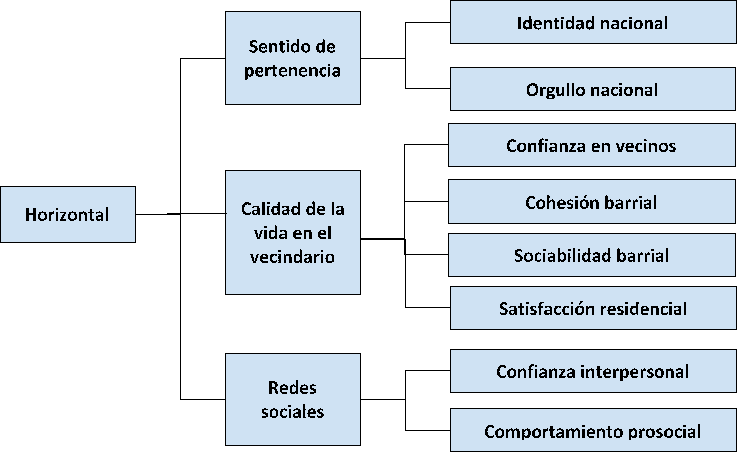
\includegraphics{inputs/images/horizontal.png}

\hypertarget{vertical}{%
\section{Vertical}\label{vertical}}

La dimensión vertical está dirigida hacia la cohesión entre los ciudadanos (o sociedad civil) y el Estado y posee indicadores subjetivos y objetivos. Los indicadores subjetivos miden la confianza de las personas hacia las principales autoridades públicas y hacia las instituciones políticas y sociales, mientras que los indicadores objetivos están asociados con las conductas de las personas, a partir de la participación política.

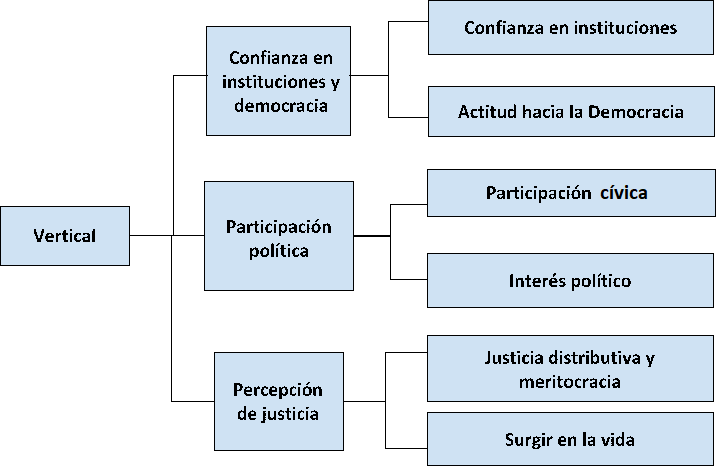
\includegraphics{inputs/images/vertical.png}

\hypertarget{bibliografuxeda}{%
\chapter*{Bibliografía}\label{bibliografuxeda}}
\addcontentsline{toc}{chapter}{Bibliografía}

\hypertarget{refs}{}
\leavevmode\hypertarget{ref-castillo_Conceptos_2021}{}%
Castillo, J., Olivos, F., \& Iturra, J. (2021). \emph{Conceptos y medición de cohesión social en proyectos internacionales. Serie Documentos de Trabajo COES, Documento de trabajo N47, pp. 1-32.}

\leavevmode\hypertarget{ref-chan_Reconsidering_2006}{}%
Chan, J., To, H.-P., \& Chan, E. (2006). Reconsidering Social Cohesion: Developing a Definition and Analytical Framework for Empirical Research. \emph{Social Indicators Research}, \emph{75}(2), 273--302. \url{https://doi.org/10.1007/s11205-005-2118-1}

\end{document}
